\documentclass[a4paper,12pt]{article} 
\usepackage[T1]{fontenc}              
\usepackage[frenchb]{babel} % césures, titres français
\usepackage[utf8]{inputenc} % encodage
\usepackage[a4paper,left=3cm,right=3cm,top=2cm,bottom=2cm]{geometry} % marges
\usepackage{graphicx} % insertion d'images
\usepackage{rotating}
\usepackage{float} % permet d'utiliser H pour placer un flottant obligatoirement
\usepackage{pdfpages} % inclusion de PDF au sein du document
\usepackage{listings}
\pagestyle{plain} % pied de pages simples

\setlength{\parskip}{1ex plus 0.5ex minus 0.2ex} % espace entre les paragraphes
\setcounter{tocdepth}{2}
\setcounter{secnumdepth}{2}

\lstset{% general command to set parameter(s)
basicstyle=\ttfamily, % print whole listing small
keywordstyle=\color{black}\bfseries\underbar,
% underlined bold black keywords
identifierstyle=, % nothing happens
commentstyle=\color{white}, % white comments
showstringspaces=false,
numbers=left,
language=java,
breaklines=true,
frame=tblr} % no special string spaces

%%%% debut macro %%%%
\makeatletter
\renewcommand\section{\@startsection {section}{1}{\z@}%
                           {-3.5ex \@plus -1ex \@minus -.2ex}%
                           {2.3ex \@plus.2ex}%
                           {\normalfont\Large\bfseries}}
\makeatother
%%%% fin macro %%%%



% Def
\newcommand{\code}[1]{{\lstinline{#1}}}

\begin{document}
\newpage
\title{TP Sécurité des réseaux}
\author{BRIZAI Olivier\\THORAVAL Maxime}
\maketitle

\newpage
\tableofcontents
\newpage


\section{Introduction}
Le but de ce TP est de mettre en place un réseau sécurisé à l'aide d'un firewall CISCO ASA.\\
Ci-dessous, le réseau que nous souhaitons obtenir (les règles de filtrage ne sont pas représentées).

\begin{figure}[H]
	\center
	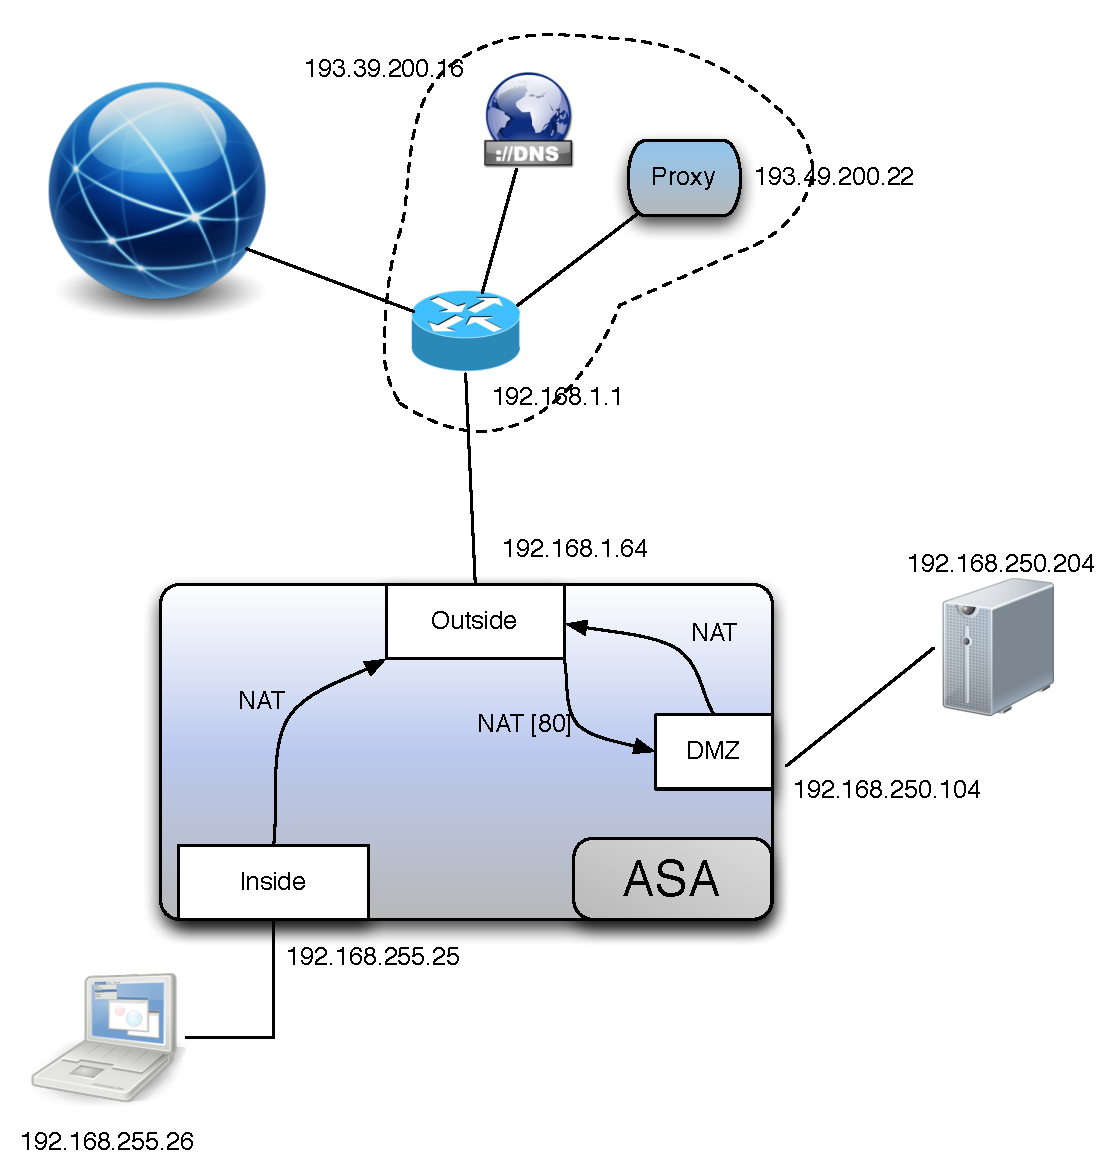
\includegraphics[width=15cm]{img/reseau.pdf}
	\caption{Réseau à obtenir}
\end{figure}

\newpage




\section{Installation et Configurations préliminaires}
\subsection{Client}
Dans un premier temps, nous avons installé Ubuntu 9.04 (version client) sur le PC relié à l'interface \textit{inside}. Celle-ci effectuée, nous réalisons les démarches suivantes, c'est à dire mise en place de Java ainsi que l'installation du paquet \og Minicom \fg.\\
Nous lançons ensuite la commande \textbf{minicom -s} et définissons les divers paramètres afin de configurer le port console. Puis, nous définissons l'adresse \textit{inside} de l'ASA. Nous pouvons maintenant, à partir de celle-ci, accéder à l'interface d'administration de l'ASA au sein de notre navigateur.\\La figure ci-dessous présente l'accueil de celle-ci. 

\begin{figure}[H]
	\center
	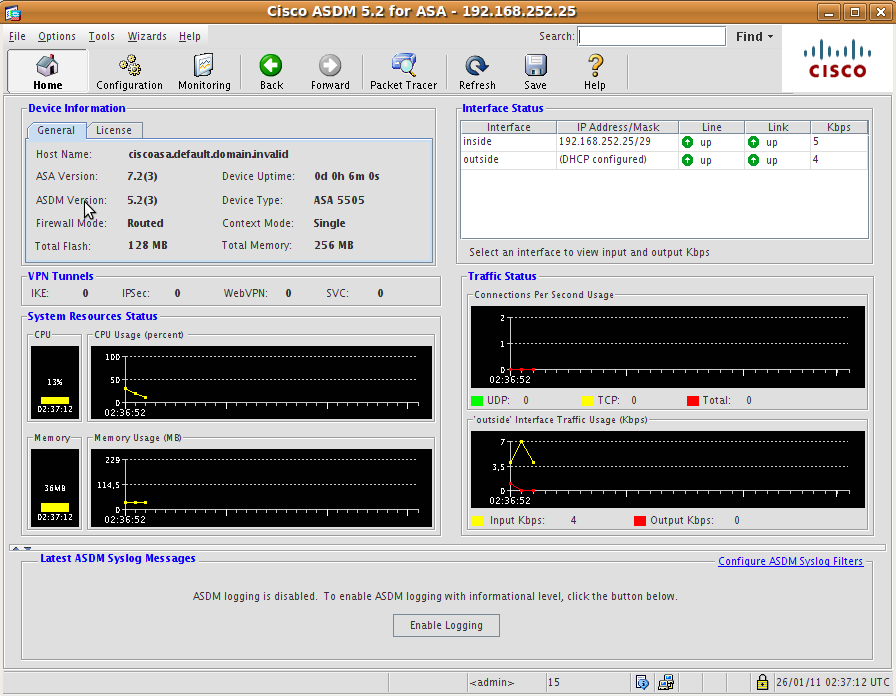
\includegraphics[width=15cm]{img/1-Interfaceconfigfw.png}
	\caption{Interface de configuration}
\end{figure}

Nous avons ensuite utilisé le \og Wizard \fg de l'application pour mettre en place un certain nombres de paramètres tel que adresses IP (inside, outside, dmz) ou encore la répartition des interfaces du firewall (cf. figure ci-dessous). 
\begin{figure}[H]
	\center
	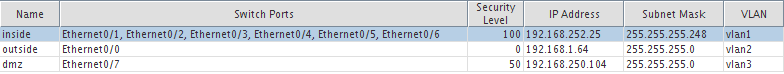
\includegraphics[width=15cm]{img/2-Interfaces.png}
	\caption{Configuration des interfaces}
\end{figure}

Enfin, nous mettons en place une route statique sur l'interface \textit{outside} afin que tous les paquets provenant des autres interfaces soit envoyés par
défaut à la passerelle de l'ENSICAEN.
\begin{figure}[H]
	\center
	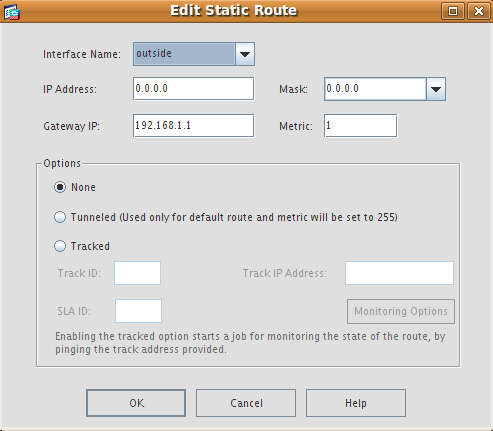
\includegraphics[width=10cm]{img/2-statiqueroute.png}
	\caption{Route statique}
\end{figure}


\subsection{Serveur}
En parallèle, nous installons \og Ubuntu 9.0.4 server \fg{} sur le PC relié à l'interface \textit{dmz} du firewall. Lors de l'installation, nous indiquons que nous souhaitons avoir par défaut les services suivants : un serveur SSH et un serveur web (LAMP).

L'installation terminée, nous allons maintenant configurer les informations réseau de notre serveur. Nous renseignons son adresse IP (192.168.250.204), le masque associé et enfin le routeur (ici il s'agit de l'adresse de l'interface \textit{dmz} de notre firewall).\\
Afin de mettre en place ces informations, nous allons modifier le fichier \textit{/etc/network/interfaces} de la sorte :
\begin{lstlisting}
auto eth0 
iface eth0 inet static
    address 192.168.250.204
    netmask 255.255.255.0
    gateway 192.168.250.104
\end{lstlisting}






\newpage
\section{Configuration Inside}
Dans cette partie, nous avons configuré notre firewall afin de permettre certaines actions au sous réseau relié à l'interface \textit{inside}.

\subsection{Configuration du NAT}
Dans un premier temps, il nous a fallu configurer une règle de NAT afin de traduire l'adresse privée de l'interface \textit{inside} en l'adresse publique de
l'interface \textit{outside}. Nous devons effectuer cette étape afin de réduire les adresses IP utilisées, d'une part dans le but de ralentir la pénurie d'adresse
IPv4, mais aussi pour que la passerelle de l'ENSICAEN c'est qu'une adresse à gérer (celle définie à l'interface \textit{outside}).

Un NAT a pour effet de remplacer les adresses sources des paquets provenant d'un réseau (ou PC) par celle souhaitée (ici remplacement de celles du sous-réseau \textit{inside} par \textit{outside}). Pour les paquets retours (exemple paquet acquitant la réception), le firewall va pouvoir le transmettre
au bon destinataire grâce à une sauvegarde de la transaction.

Ci-dessous, la configuration de notre NAT, pour le sous-réseau de lié à notre interface \textit{inside} (192.168.252.24), nous lions l'adresse de l'interface \textit{outside}.
\begin{figure}[H]
	\center
	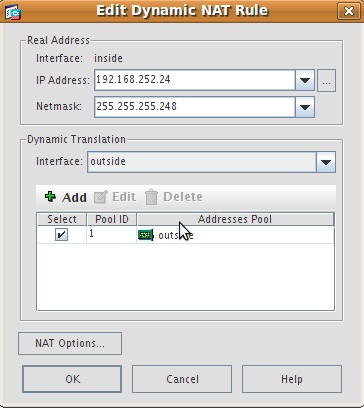
\includegraphics[width=10cm]{img/3-natinsideoutside.png}
	\caption{Configuration du NAT}
\end{figure}


\subsection{Règles de filtrage}
Notre NAT crée, nous allons maintenant mettre en place des règles de filtrage afin de ne laisser passer que les paquets liés à des services définis.
Il faut savoir que lorsque des paquets TCP et UDP sont envoyés, une connexion est établie. Cela permet de n'avoir à définir que les règles de sortie, celles
d'entrées étant liées. Nous pourrons remarquer que le port source des règles est toujours définis sur \og Any \fg{}, en effet, l'application effectuant la demande
n'utilise pas forcément le port dédié.

Chaque règle appliquées ici autorise les services à tout le sous réseau connecté à l'interface \textit{inside}. Il aurait, par exemple, pu être possible de
réduire l'accès au service SSH qu'à certaines machines mais nous pensons que ce n'est pas nécessaire dans le cadre de notre TP.

Dans un premier temps, nous autorisations les flux TCP et UDP sur le port 53 (DOMAIN) qui sont à destination de 193.49.200.16 (adresse du serveur DNS de
l'ENSICAEN).

\begin{figure}[H]
	\center
	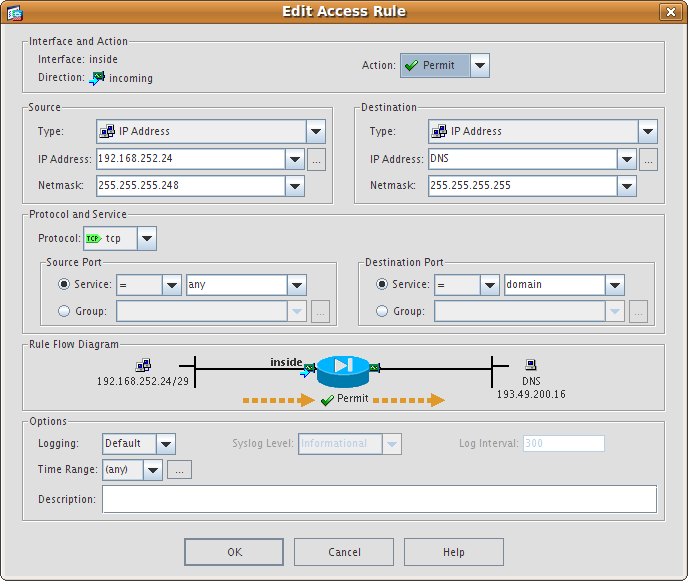
\includegraphics[width=13cm]{img/4-policyinsidednstcp.png}
	\caption{Règle TCP d'accès au DNS}
\end{figure}
\begin{figure}[H]
	\center
	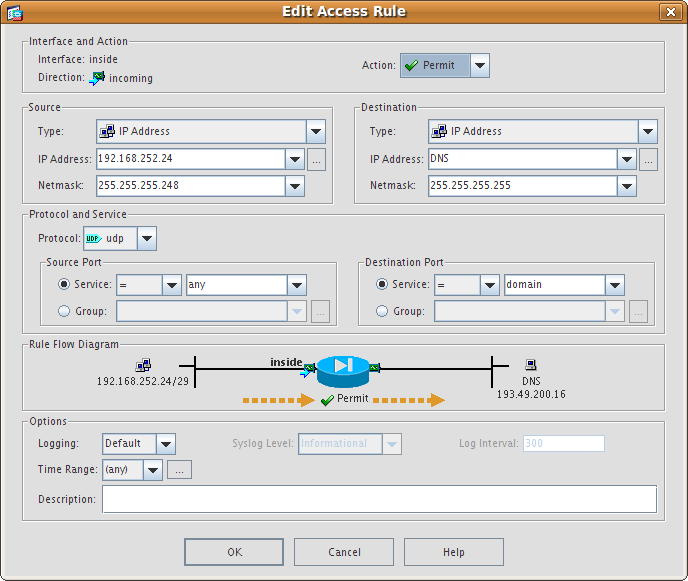
\includegraphics[width=13cm]{img/5-policyinsidednsudp.png}
	\caption{Règle UDP d'accès au DNS}
\end{figure}


\newpage
Maintenant, nous créons la règle autorisant le flux SSH (TCP sur le port 22). Nous ne nous soucions pas de la cible de la demande.
\begin{figure}[H]
	\center
	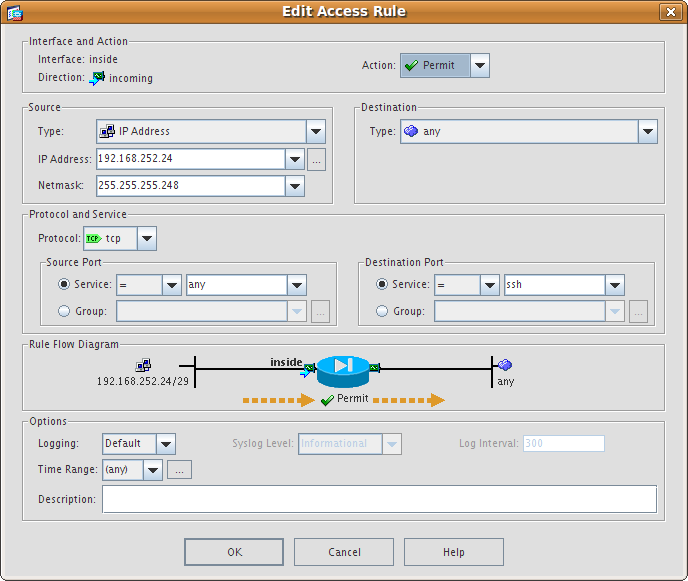
\includegraphics[width=15cm]{img/6-policyinsideanyssh.png}
	\caption{Règle SSH}
\end{figure}


\newpage
Puis la règle autorisant le flux HTTP (TCP sur le port 80) à destination de n'importe quelle machine.
\begin{figure}[H]
	\center
	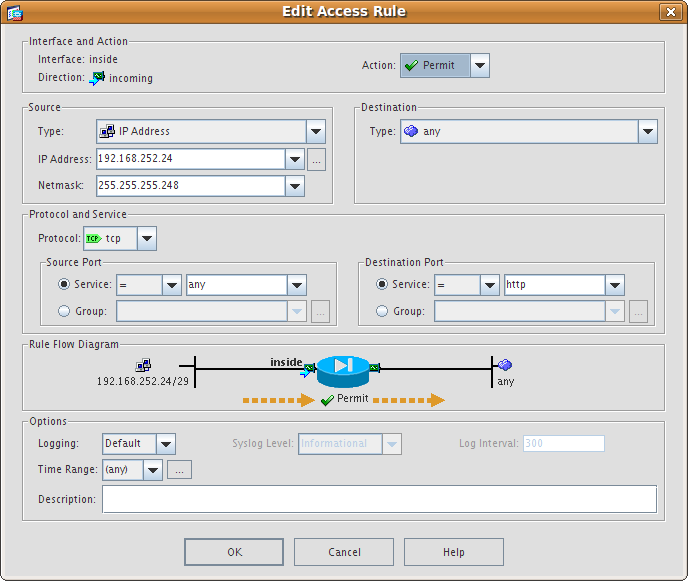
\includegraphics[width=15cm]{img/7-policyinsidehttpany.png}
	\caption{Règle HTTP}
\end{figure}


\newpage
Enfin, nous autorisons le flux à destination d'un proxy (TCP sur le port 3128 = port du proxy de l'école). Bien entendu, nous nous restreignons à l'adresse du
proxy de l'ENSICAEN. 
\begin{figure}[H]
	\center
	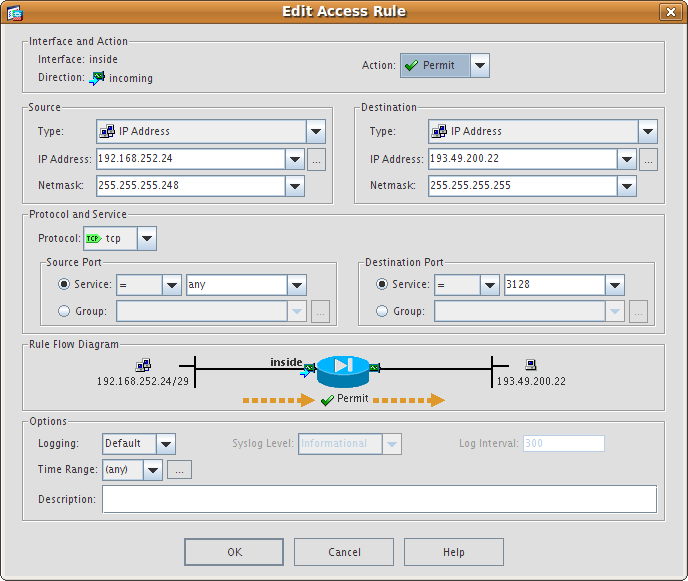
\includegraphics[width=15cm]{img/8-policyinsidetcpproxy.png}
	\caption{Règle Proxy}
\end{figure}


\newpage
\subsubsection{Problèmes rencontrés}
\textit{Ping}

Nous sommes maintenant censé pouvoir accéder au routeur de l'école (adresse 192.168.1.1). Pour le vérifier, nous lançons la commande \textbf{ping} sur son adresse. On remarque que nous n'avons pas de retour de cette commande. Afin de vérifier l'erreur, nous allons regarder le \textit{monitoring} de notre firewall. Ceci va nous permettre de suivre son activité. Après analyse des traces, nous avons pu comprendre l'échec de la commande \textbf{ping}. En effet, elles nous informent que les paquets de type ICMP ne sont pas autorisés à destination de l'interface \textit{inside}. Afin de résoudre ce problème, nous devons rajouter une nouvelle règle de filtrage que nous avons défini de la manière ci-dessous.
\begin{figure}[H]
	\center
	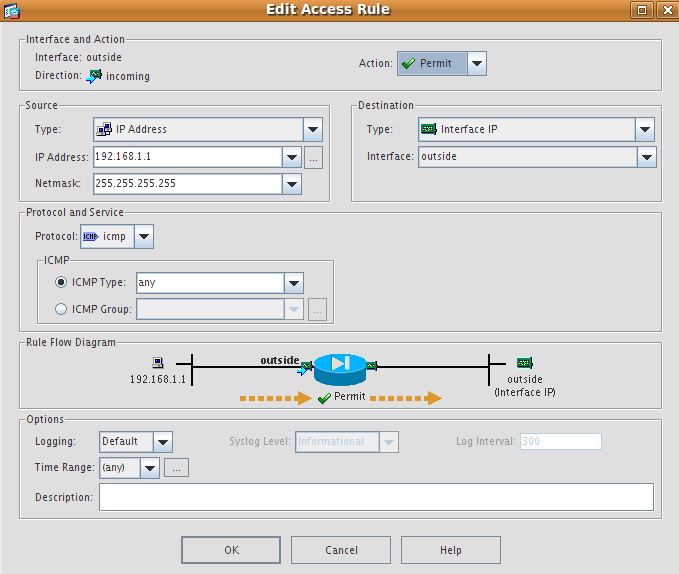
\includegraphics[width=12cm]{img/9-Pingrevientpasflitrageicmp.png}
	\caption{Filtrage ICMP pour autoriser le retour de ping}
\end{figure}

Cette règle mise en place, nous lançons une nouvelles fois la commande \textbf{ping}. Comme visible sur la figure ci-dessous, il n'y a plus d'échec.
\begin{figure}[H]
	\center
	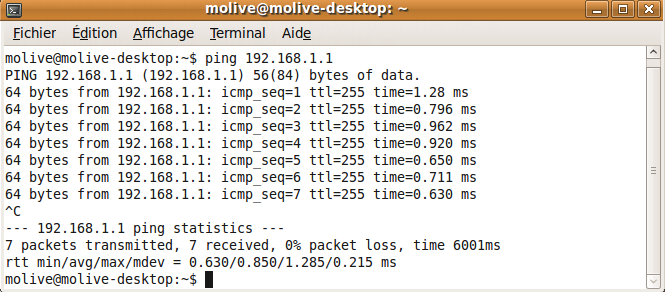
\includegraphics[width=11cm]{img/10-pingok.png}
	\caption{Résultat ping}
\end{figure}

~

\textit{Utilisation du DNS}

La règle du DNS étant active, nous considérions que l'ordinateur branché sur \textit{inside} pouvait accéder à son service. Pour le vérifier, nous avons
essayer plusieurs commandes listées ci-dessous
\begin{lstlisting}
ping google.fr
host google.fr
nslookup google.fr
\end{lstlisting}

Chacune de ses commandes ne fonctionnaient pas, en effet, elles indiquaient qu'elle n'arrivait pas à récupérer l'adresse IP lié au nom de domaine. Etant
donnée que c'est au DNS de nous fournir ces informations, nous avons conclu qu'il y avait un problème de configuration. Pour tester si notre règle de 
filtrage fonctionnait, nous avons effectué ceci
\begin{lstlisting}
	telnet 193.49.200.16 53
	Trying 193.49.200.16...
	Connected to ns.ecole.ensicaen.fr.
	Escape character is '^]'.
\end{lstlisting}

Nous testons la connexion au serveur DNS sur le port 53 (comme définis dans nos règles). Nous remarquons que nous avons pu nous y connecter. (les messages
suivants sont dû au fait que nous utilisions \textbf{telnet} pour nous connecter). Nos règles sont donc fonctionnelles. Afin de vérifier l'utilisation du DNS,
nous avons fait ceci
\begin{lstlisting}
nslookup
> server 193.49.200.16
Default server: 193.49.200.16
Address: 193.49.200.16#53
> google.fr
Server:		193.49.200.16
Address:	193.49.200.16#53

Non-authoritative answer:
Name:	google.fr
Address: 209.85.229.99
Name:	google.fr
Address: 209.85.229.147
Name:	google.fr
Address: 209.85.229.104
\end{lstlisting}

Dans un premier temps, nous indiquons à \textbf{nslookup} l'adresse IP du serveur DNS. Puis, re-testons avec le nom de domaine \textit{google.fr}.
Nous pouvons voir qu'il y a un retour, le DNS est donc utilisable. Après recherche, il se trouve que c'est dans le système Linux en lui-même que 
nous avions oublié d'indiquer l'adresse IP du serveur DNS au moment de rentrer celle de la machine.


\newpage
\section{Configuration DMZ}
Maintenant que la configuration du PC client est mis en place et fonctionnelle, nous allons configurer notre serveur. Celui-ci doit être accessible de 
l'extérieur en HTTP et SSH, mais aussi par notre PC client.

\subsection{Configuration du NAT}
Comme pour l'interface \textit{inside}, nous allons définir une NAT afin de traduire les adresses du sous réseau. Etant donné que nous n'avons qu'un serveur
de connecté sur l'interface \textit{dmz}, nous donnons son adresse et non celle du sous réseau.
\begin{figure}[H]
	\center
	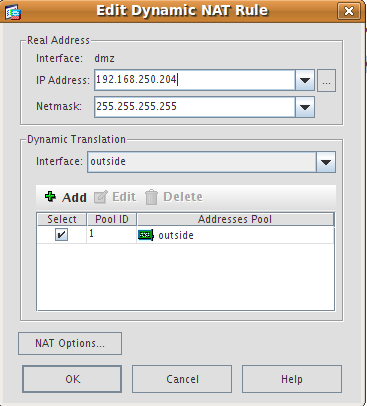
\includegraphics[width=10cm]{img/11-natdmzoutside.png}
	\caption{NAT pour l'interface \textit{dmz}}
\end{figure}

\subsection{Règles de filtrage}
Nous allons aussi autorisé quelques services à notre serveur. Pour toutes nos règles, nous allons limiter l'adresse IP source à celle de notre serveur, en effet,
c'est la seule machine du sous-réseau.

Dans un premier temps, l'accès au serveur DNS. Nous autorisons le flux TCP et UDP sur le port 53 spécifiquement pour notre serveur (192.168.250.204).
\begin{figure}[H]
	\center
	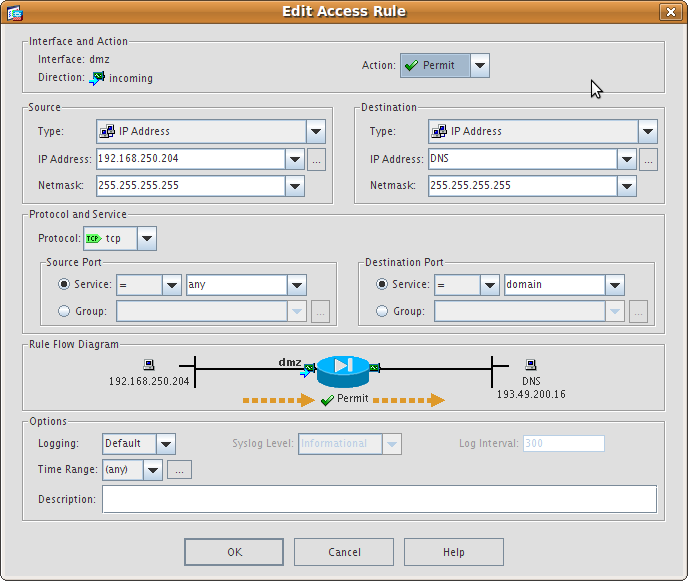
\includegraphics[width=12cm]{img/12-policydmzdnstcp.png}
	\caption{Règle TCP pour l'accès au DNS}
\end{figure}
\begin{figure}[H]
	\center
	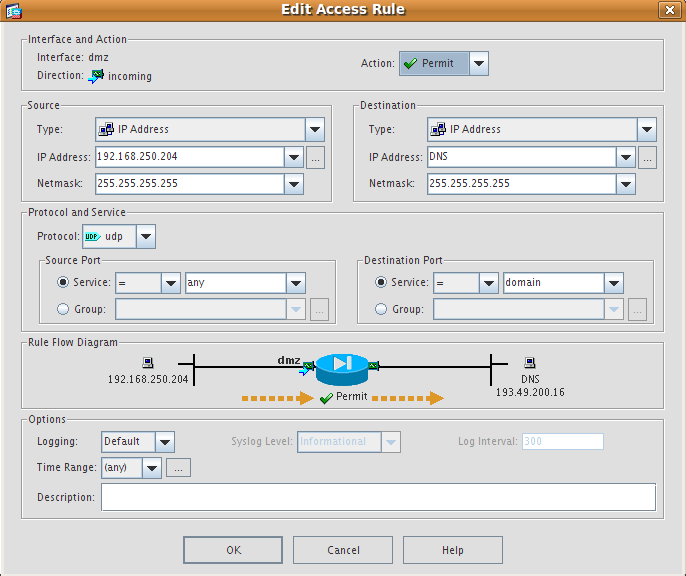
\includegraphics[width=12cm]{img/12-policydmzdnsudp.png}
	\caption{Règle UDP pour l'accès au DNS}
\end{figure}

Nous devons aussi indiquer au système l'adresse du serveur DNS. Pour ce faire, nous éditons le fichier \textit{/etc/resolv.conf} de cette manière.
\begin{lstlisting}
	nameserver 193.49.200.16
\end{lstlisting}

Nous autorisons aussi le flux HTTP et SSH en sortie, tout comme pour l'interface \textit{inside}.
\begin{figure}[H]
	\center
	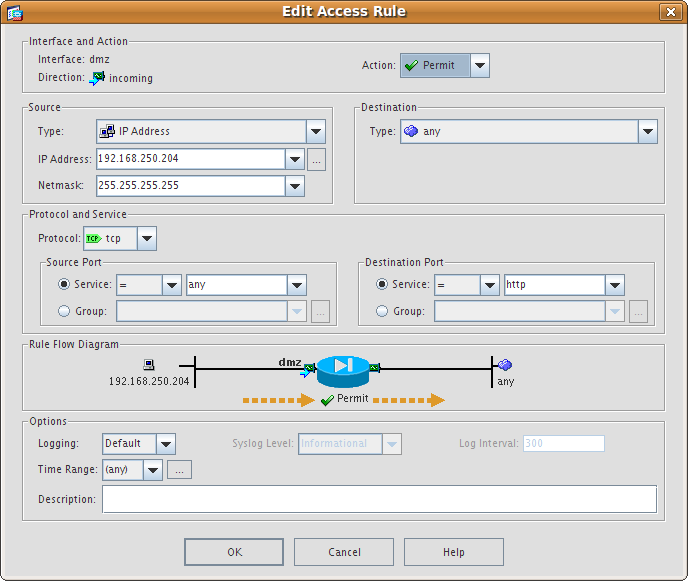
\includegraphics[width=12cm]{img/13-policydmzhttpany.png}
	\caption{Règle HTTP}
\end{figure}
\begin{figure}[H]
	\center
	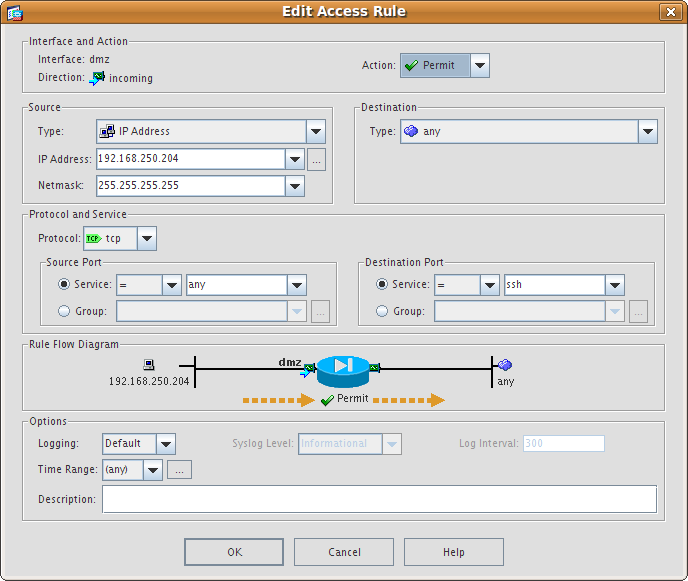
\includegraphics[width=12cm]{img/14-policydmzsshany.png}
	\caption{Règle SSH}
\end{figure}

Nous donnons aussi l'autorisation d'envoyer des paquets en direction du proxy de l'ENSICAEN.
\begin{figure}[H]
	\center
	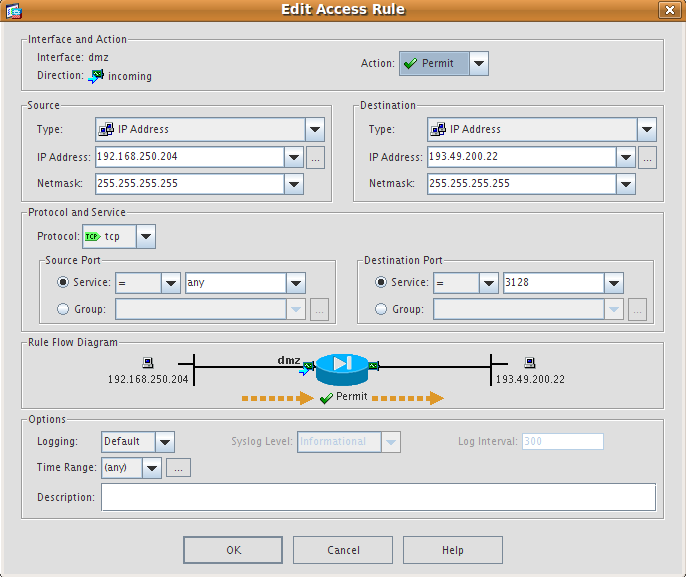
\includegraphics[width=12cm]{img/15-policydmzproxy.png}
	\caption{Règle d'accès au proxy}
\end{figure}

Notre serveur est maintenant capable de discuter avec l'extérieur. Notre but est de pouvoir y accéder à partir de notre client. Pour cela, nous utiliserons 
la technologie SSH. Avant de tester celle-ci, nous allons voir si notre serveur est accessible. Pour cela, nous allons utiliser la commande \textbf{ping}
une nouvelle fois à partir de notre pc client. Nous remarquons que cela ne fonctionne pas, nous ne pouvons y accéder. Les log nous indique qu'il y a un problème
de translation. Ceci est dû au NAT crée entre l'interface \textit{inside} et \textit{outside}. Afin de résoudre ceci, nous allons y créer une exception indiquant
qu'il ne faut pas traduire les messages en provenance du sous-réseau \textit{inside} à destination du serveur (192.168.250.204).

\begin{figure}[H]
	\center
	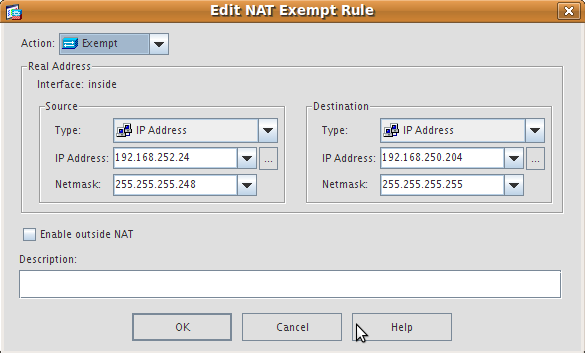
\includegraphics[width=12cm]{img/16-natexception.png}
	\caption{Exception du NAT}
\end{figure}

\subsection{HTTP et SSH à partir du réseau ENSICAEN}
Nous pouvons maintenant accéder à notre serveur à partir de notre PC que ce soit en SSH ou en HTML. Cependant, cet accès est restreint à l'interface
\textit{inside}, en effet, nous souhaiterions que des personnes reliées au serveur de l'ENSICAEN puisse accéder à nos pages web ou encore se connecter en SSH.

Dans un premier temps, nous acceptons les flux HTTP. Nous aurions pu mettre l'adresse IP de notre serveur en tant que destination, mais sachant qu'il n'y a pas
de serveur HTTP sur notre PC client, les utilisateurs n'ont aucun intérêt à aller l'interroger.
\begin{figure}[H]
	\center
	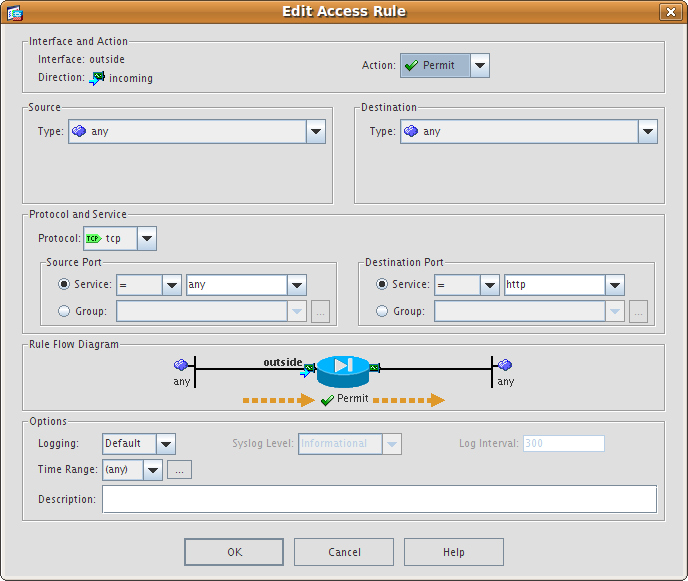
\includegraphics[width=12cm]{img/17-policyoutsidehttpany.png}
	\caption{Filtrage HTTP sur outside}
\end{figure}

Nous configurons maintenant afin qu'il puisse y avoir des demandes de connexion SSH à partir de l'extérieur. Pour plus de sécurité, nous n'avons indiqué que 
l'IP du serveur. Nous aurions aussi pu ne pas le renseigner, limitant l'accès SSH à notre client \textit{inside}.
\begin{figure}[H]
	\center
	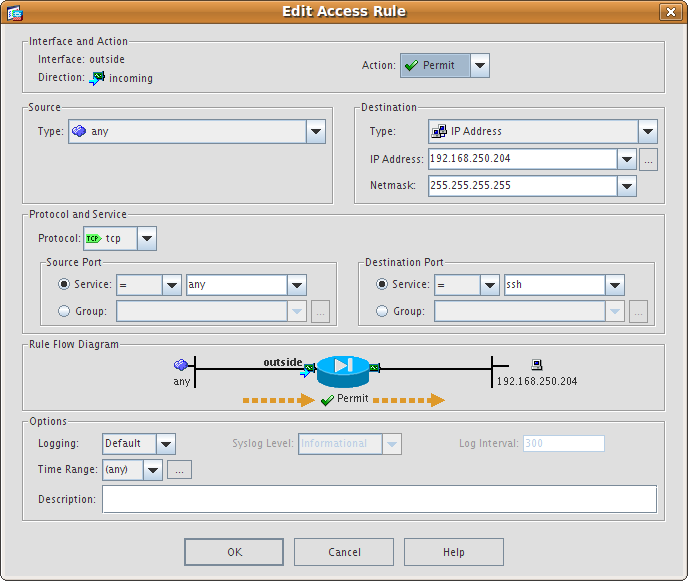
\includegraphics[width=12cm]{img/18-policyoutsidesshserver.png}
	\caption{Filtrage SSH}
\end{figure}

Il nous fallait indiquer au firewall que les flux HTTP et SSH rentrant dans l'interface \textit{dmz} doivent obligatoirement être redirigé à \textit{outside}
en utilisant son adresse. Ci-dessous, les deux NAT statiques définis pour effectuer ceci.
\begin{figure}[H]
	\center
	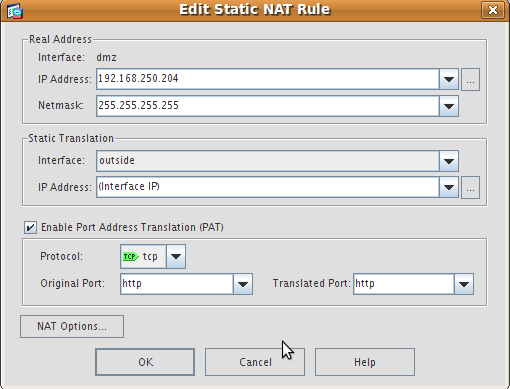
\includegraphics[width=12cm]{img/19-natstaticdmzhttp.png}
	\caption{Route statique pour HTTP}
\end{figure}

\begin{figure}[H]
	\center
	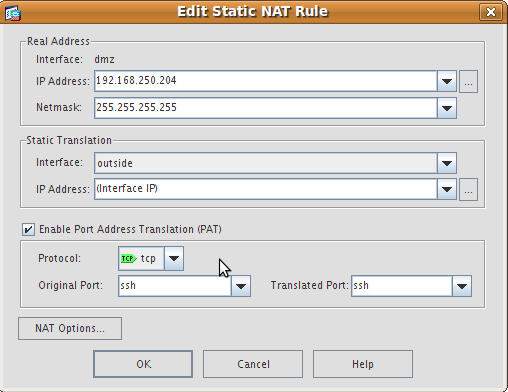
\includegraphics[width=12cm]{img/20-natstaticdmzssh.png}
	\caption{Route statique pour SSH}
\end{figure}

~

A partie de ce moment, il était possible aux personnes présentes dans le réseau ENSICAEN d'accéder à notre serveur HTTP mais aussi à se connecter en SSH.
Vous pourrez trouver en Annexe notre fichier de configuration.

\newpage
\section{Annexe}
\subsection{Configuration firewall}
\lstinputlisting{img/config_reseau} 


\end{document}




